% !TeX encoding = UTF-8
\section{Appendix}


\subsection{Example Nonce Sentences}\label{ap:nonce_sentences}

\begin{table}[H] \centering
    \begin{threeparttable}
        \begin{tabular}{ p{0.66\linewidth} c c }
            \hline
            \thead{Sentence} & \thead{Noun} & \thead{Verb} \\
            \hline\hline
            the section on current routes adds nothing to the info . & section & adds \\
            the base of the buildings contains commercial space , including two restaurants , a dental office ( pinnacle dental ) , a medical clinic , and spa , while the surrounding area will consist of public parks , shops and recreation spaces . & base & contains \\
            the genetic variation among the viruses isolated from different places ( 7-8 ) increases the difficulty of developing vaccines against it . & variation & increases \\
            the list of shipwrecks in 1980 includes all ships sunk , foundered , grounded , or otherwise lost during 1980 . & list & includes \\
            the edwardian semi-detached houses of brantwood road , facing the park have an art deco style whilst those in ashburnham road include ornate balconies . & houses & have \\
            for protestant denominations , the purposes of marriage include intimate companionship , rearing children and mutual support for both husband and wife to fulfill their life callings . & purposes & include \\
            the signs , due to being the same colour green as the shield , show a green sign with a white inlay border , and a green outer border . & signs & show \\
            the application of these techniques to humans creates moral and ethical concerns in the opinion of some , while the advantages of sensible use of selected technologies is favored by others . & application & creates \\
            under chairwoman agnes gund , the moma ps1 's board of directors includes the artists laurie anderson and paul chan , art historian diana widmaier-picasso , fashion designer adam kimmel , and art collectors richard chang , peter norton , and julia stoschek . & board & includes \\
            \hline
        \end{tabular}
        \caption{First ten sentences from the nonce dataset.} \label{Tab:nonce_sentences}
    \end{threeparttable}
\end{table}

\clearpage


\subsection{Stabilization of repeat surprisal with 10 control sequences}\label{app:rs_10_controls}

\begin{figure}[H]
  \centering
  \subfloat[\centering average surprisal by amount of control sequences for 50 randomized trials.]{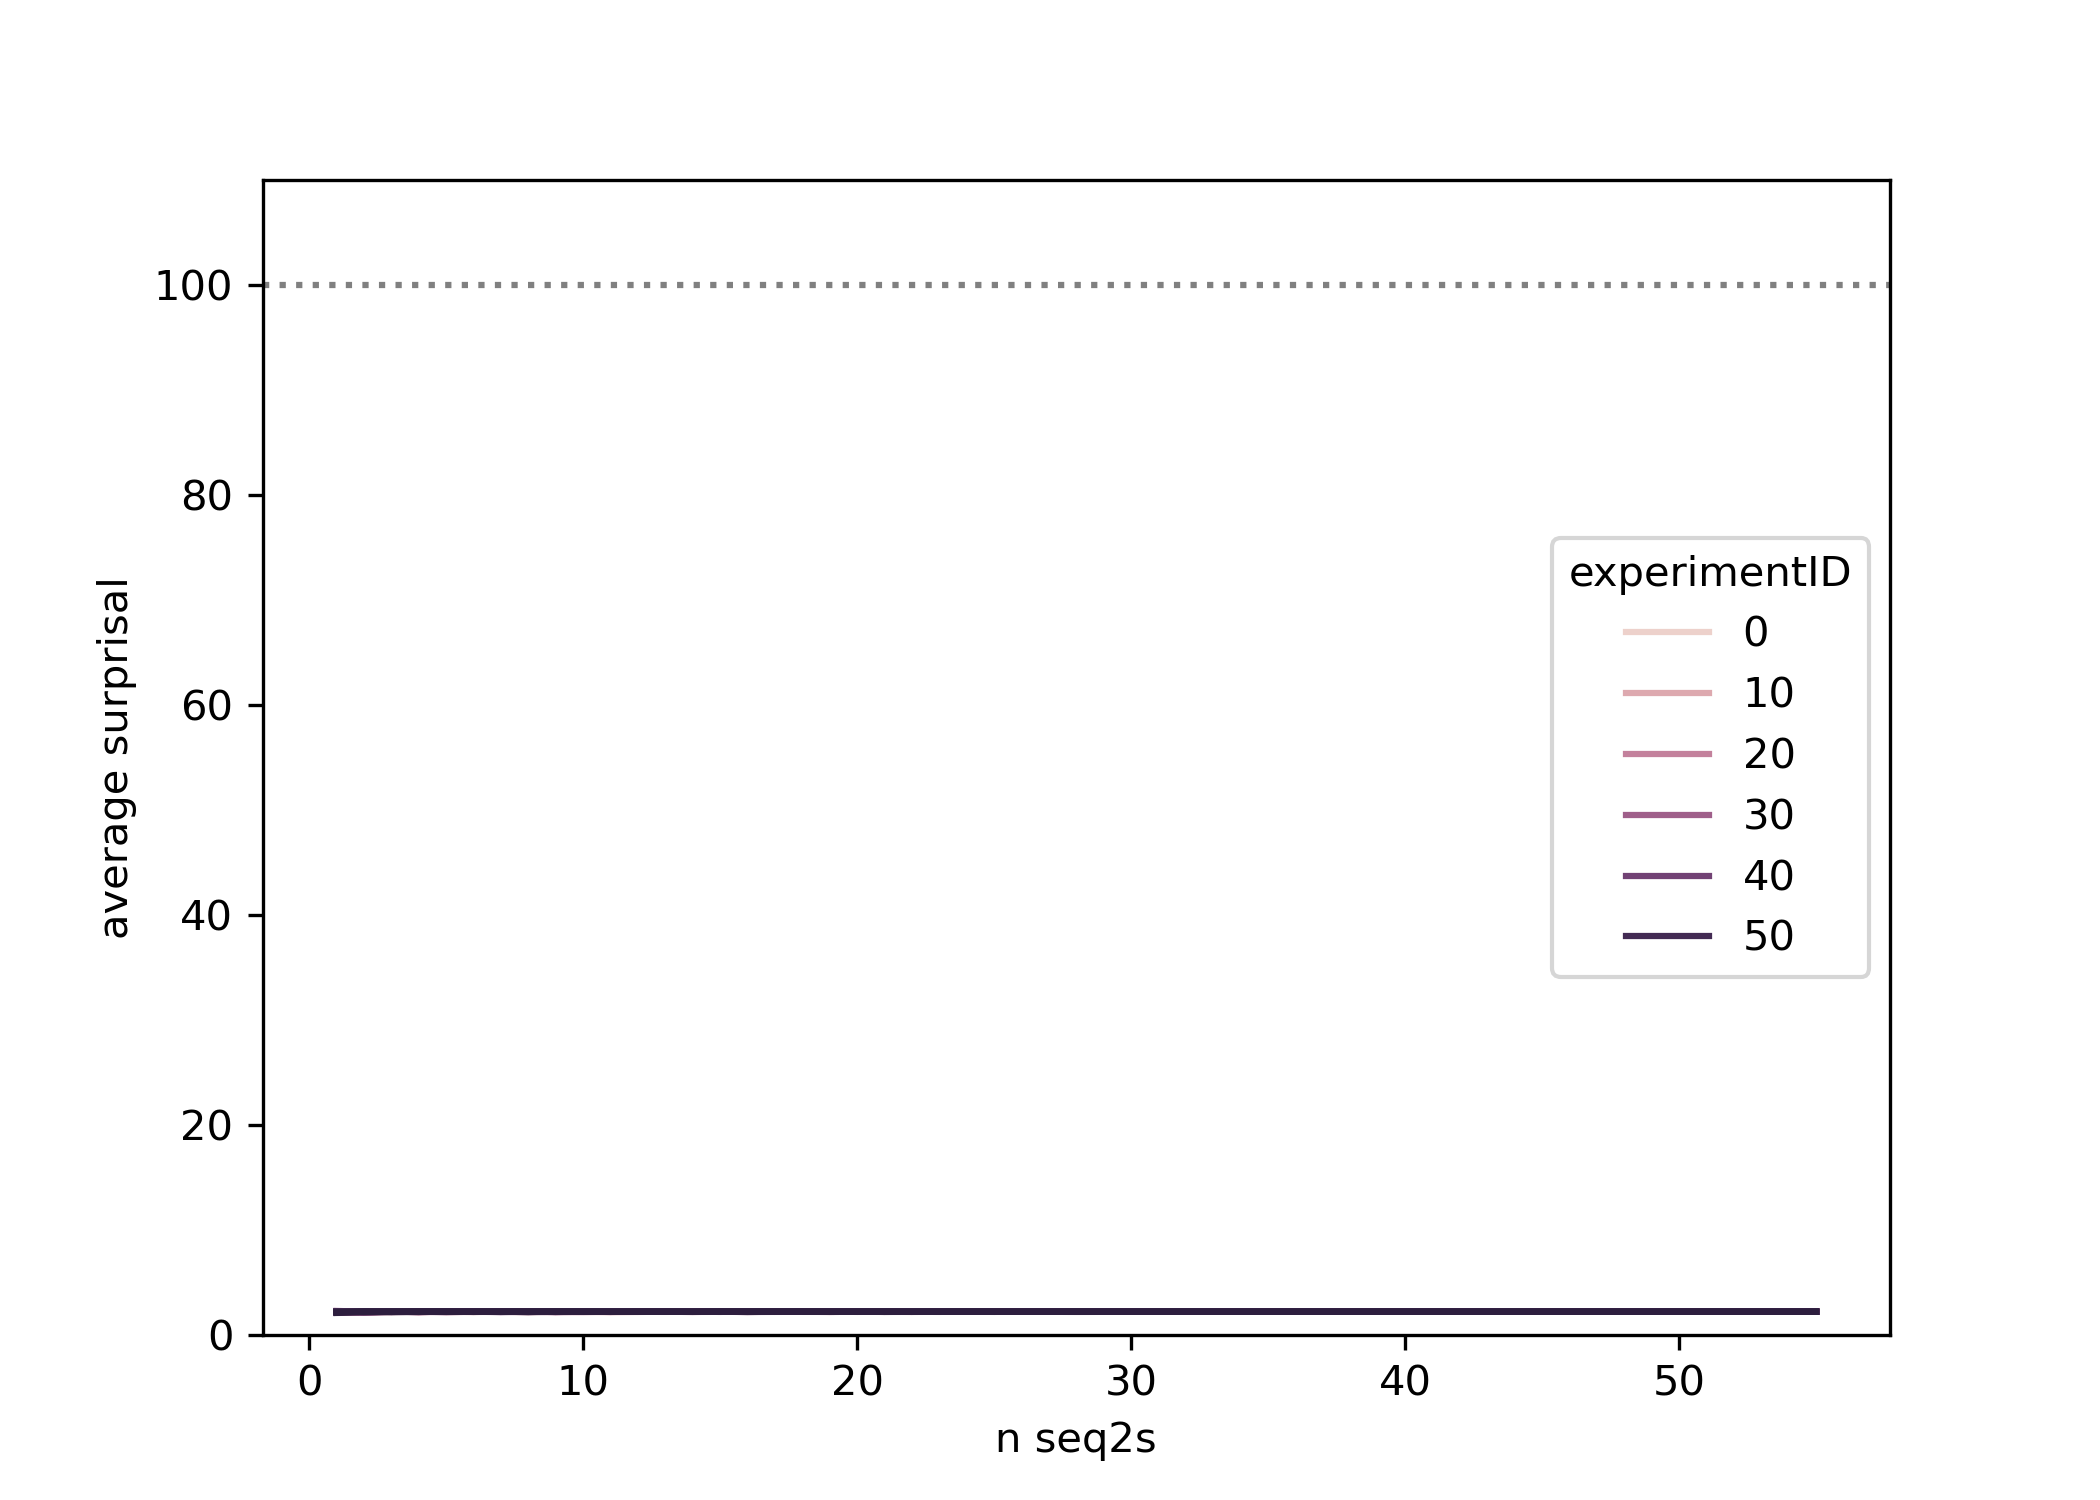
\includegraphics[width=.4\textwidth]{appendix/surprisal_nseq2.png}}\quad
  \subfloat[\centering same as (a), but scaled y-axis (surprisal) range to 2-2.4 bits]{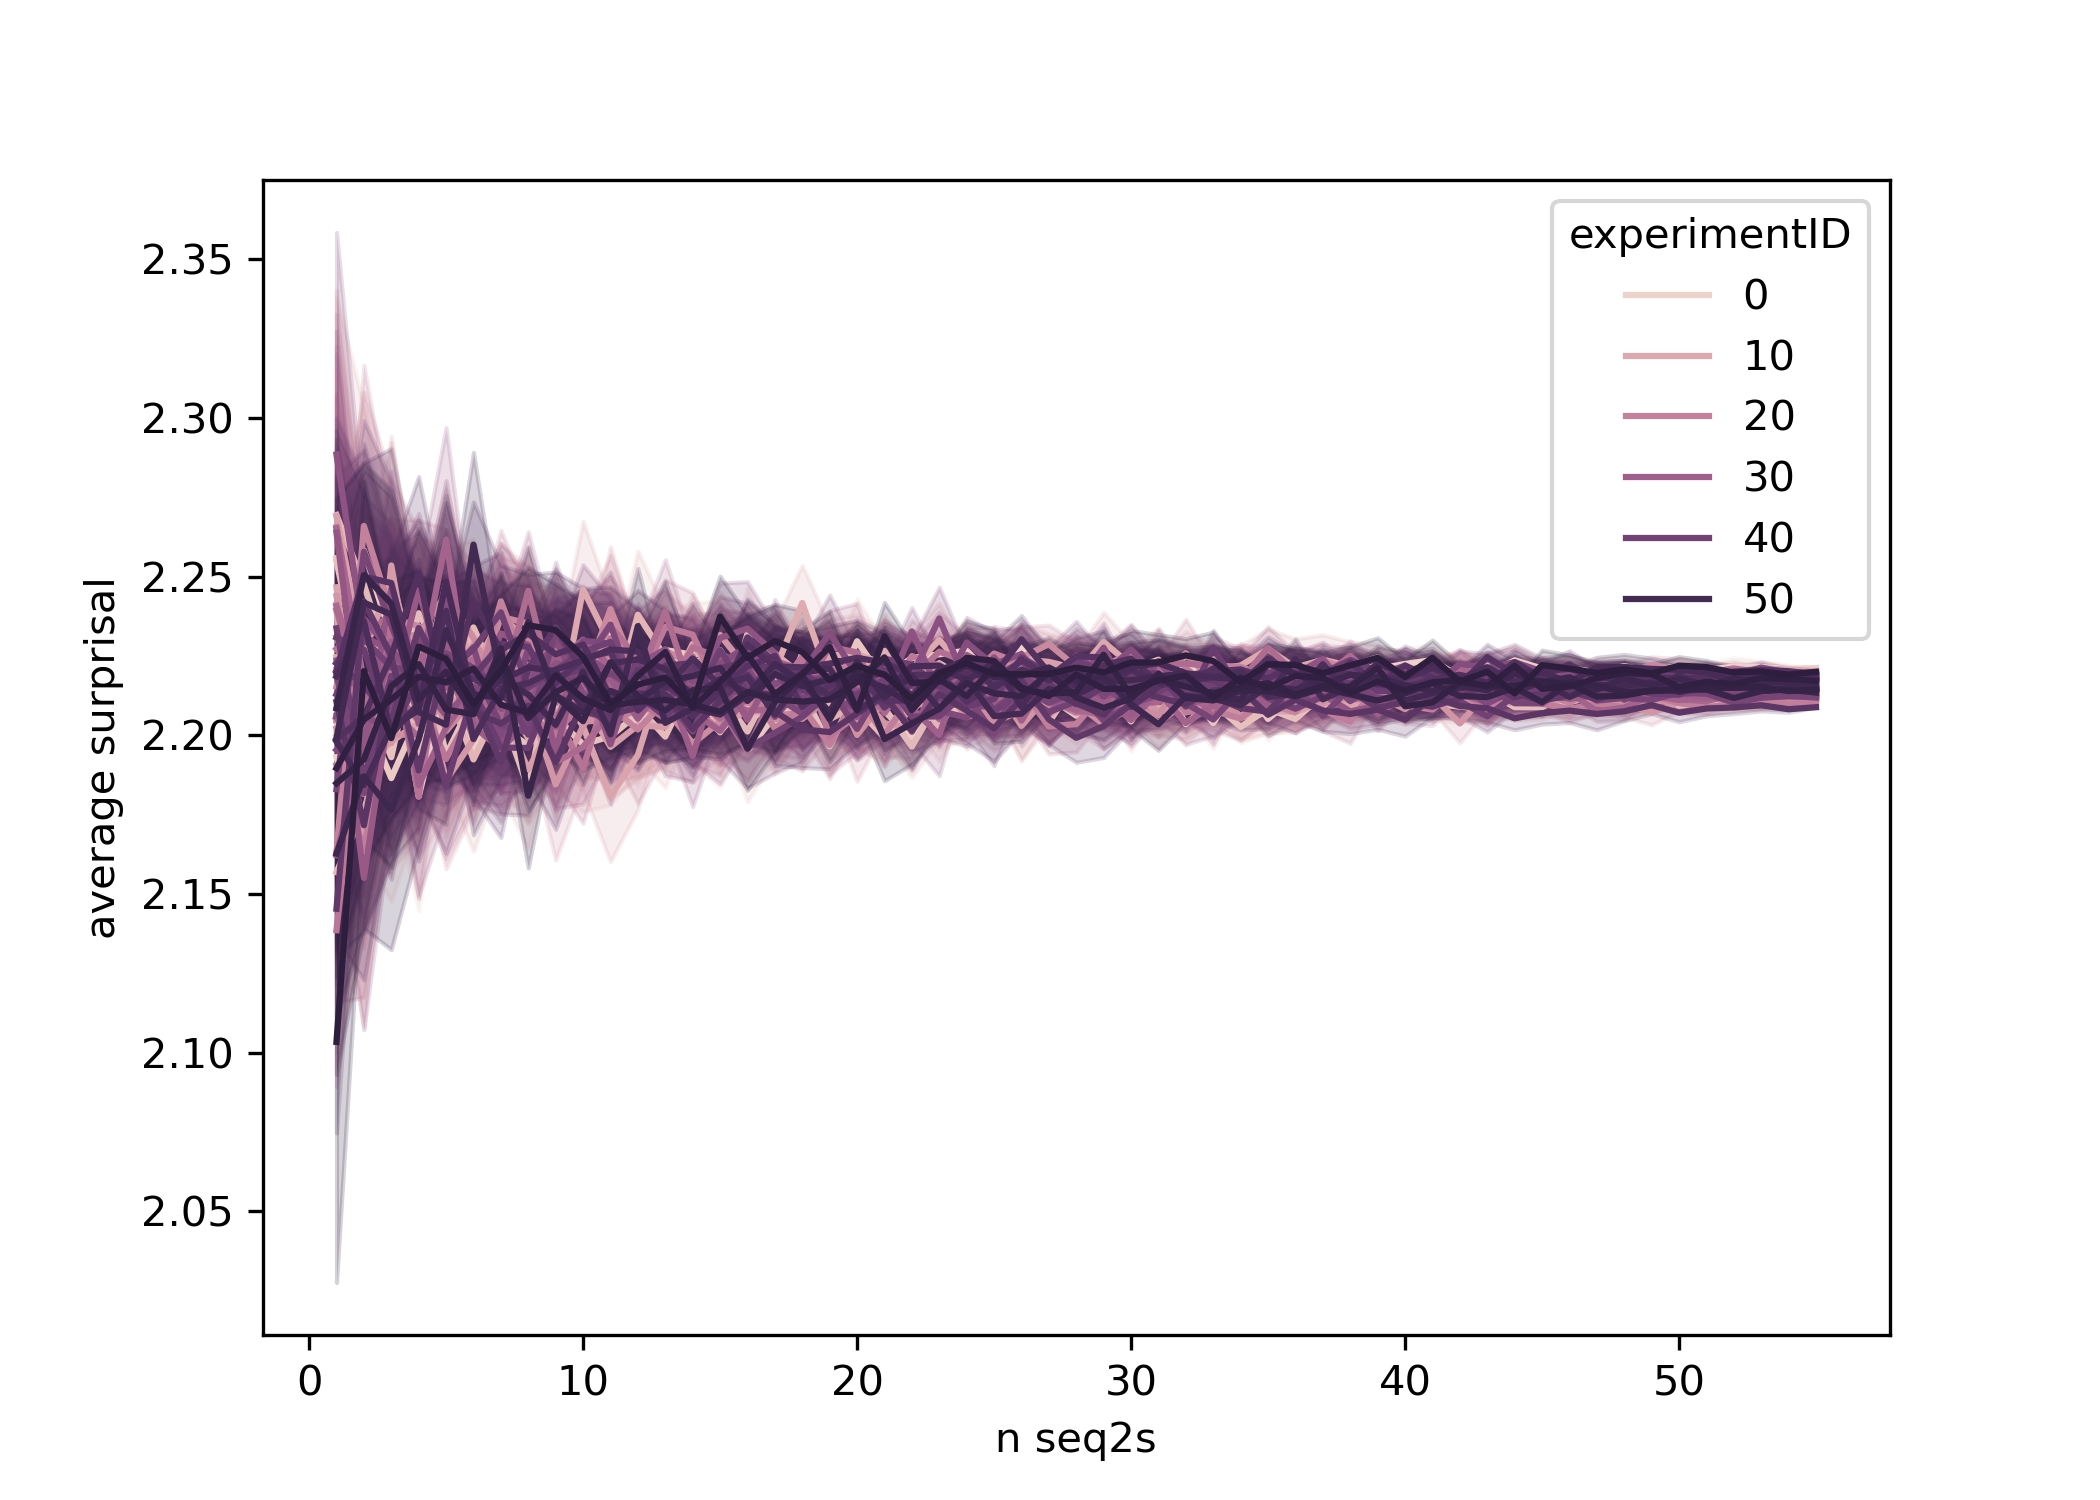
\includegraphics[width=.4\textwidth]{appendix/surprisal_nseq2_closeup.png}}\\
  \subfloat[average repeat surprisal by amount of control sequences for 50 randomized trials.]{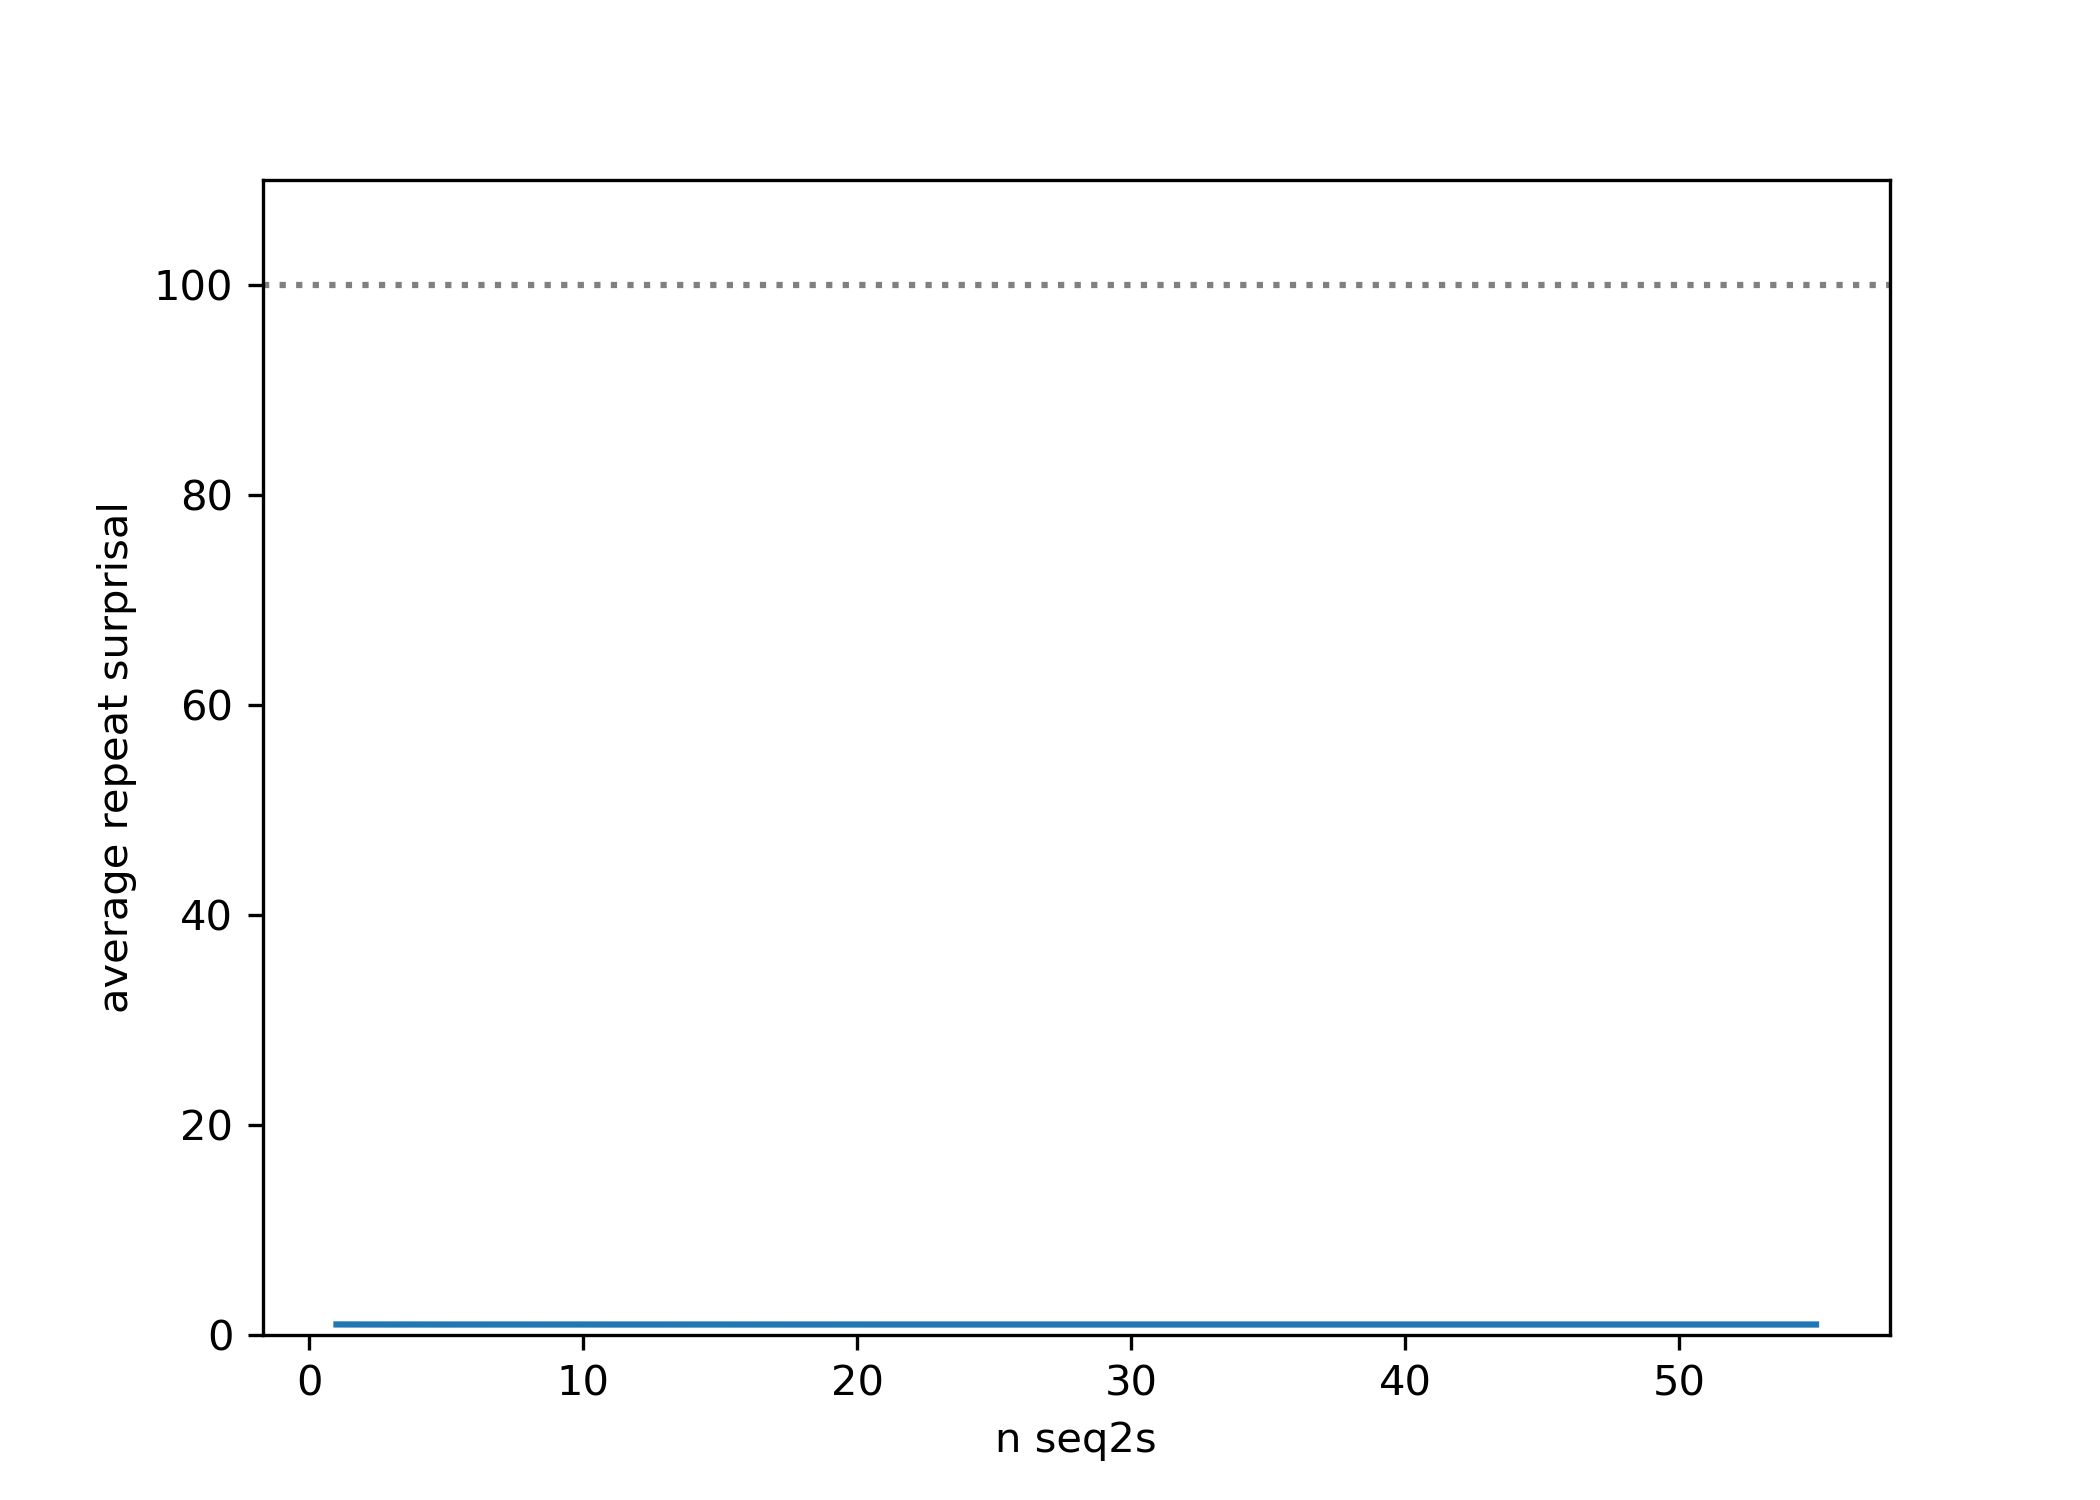
\includegraphics[width=.4\textwidth]{appendix/repeat_surprisal_nseq2.png}}\quad
  \subfloat[same as (c), but scaled y-axis (repeat surprisal) range to 0.9925  - 1.0125 percent]{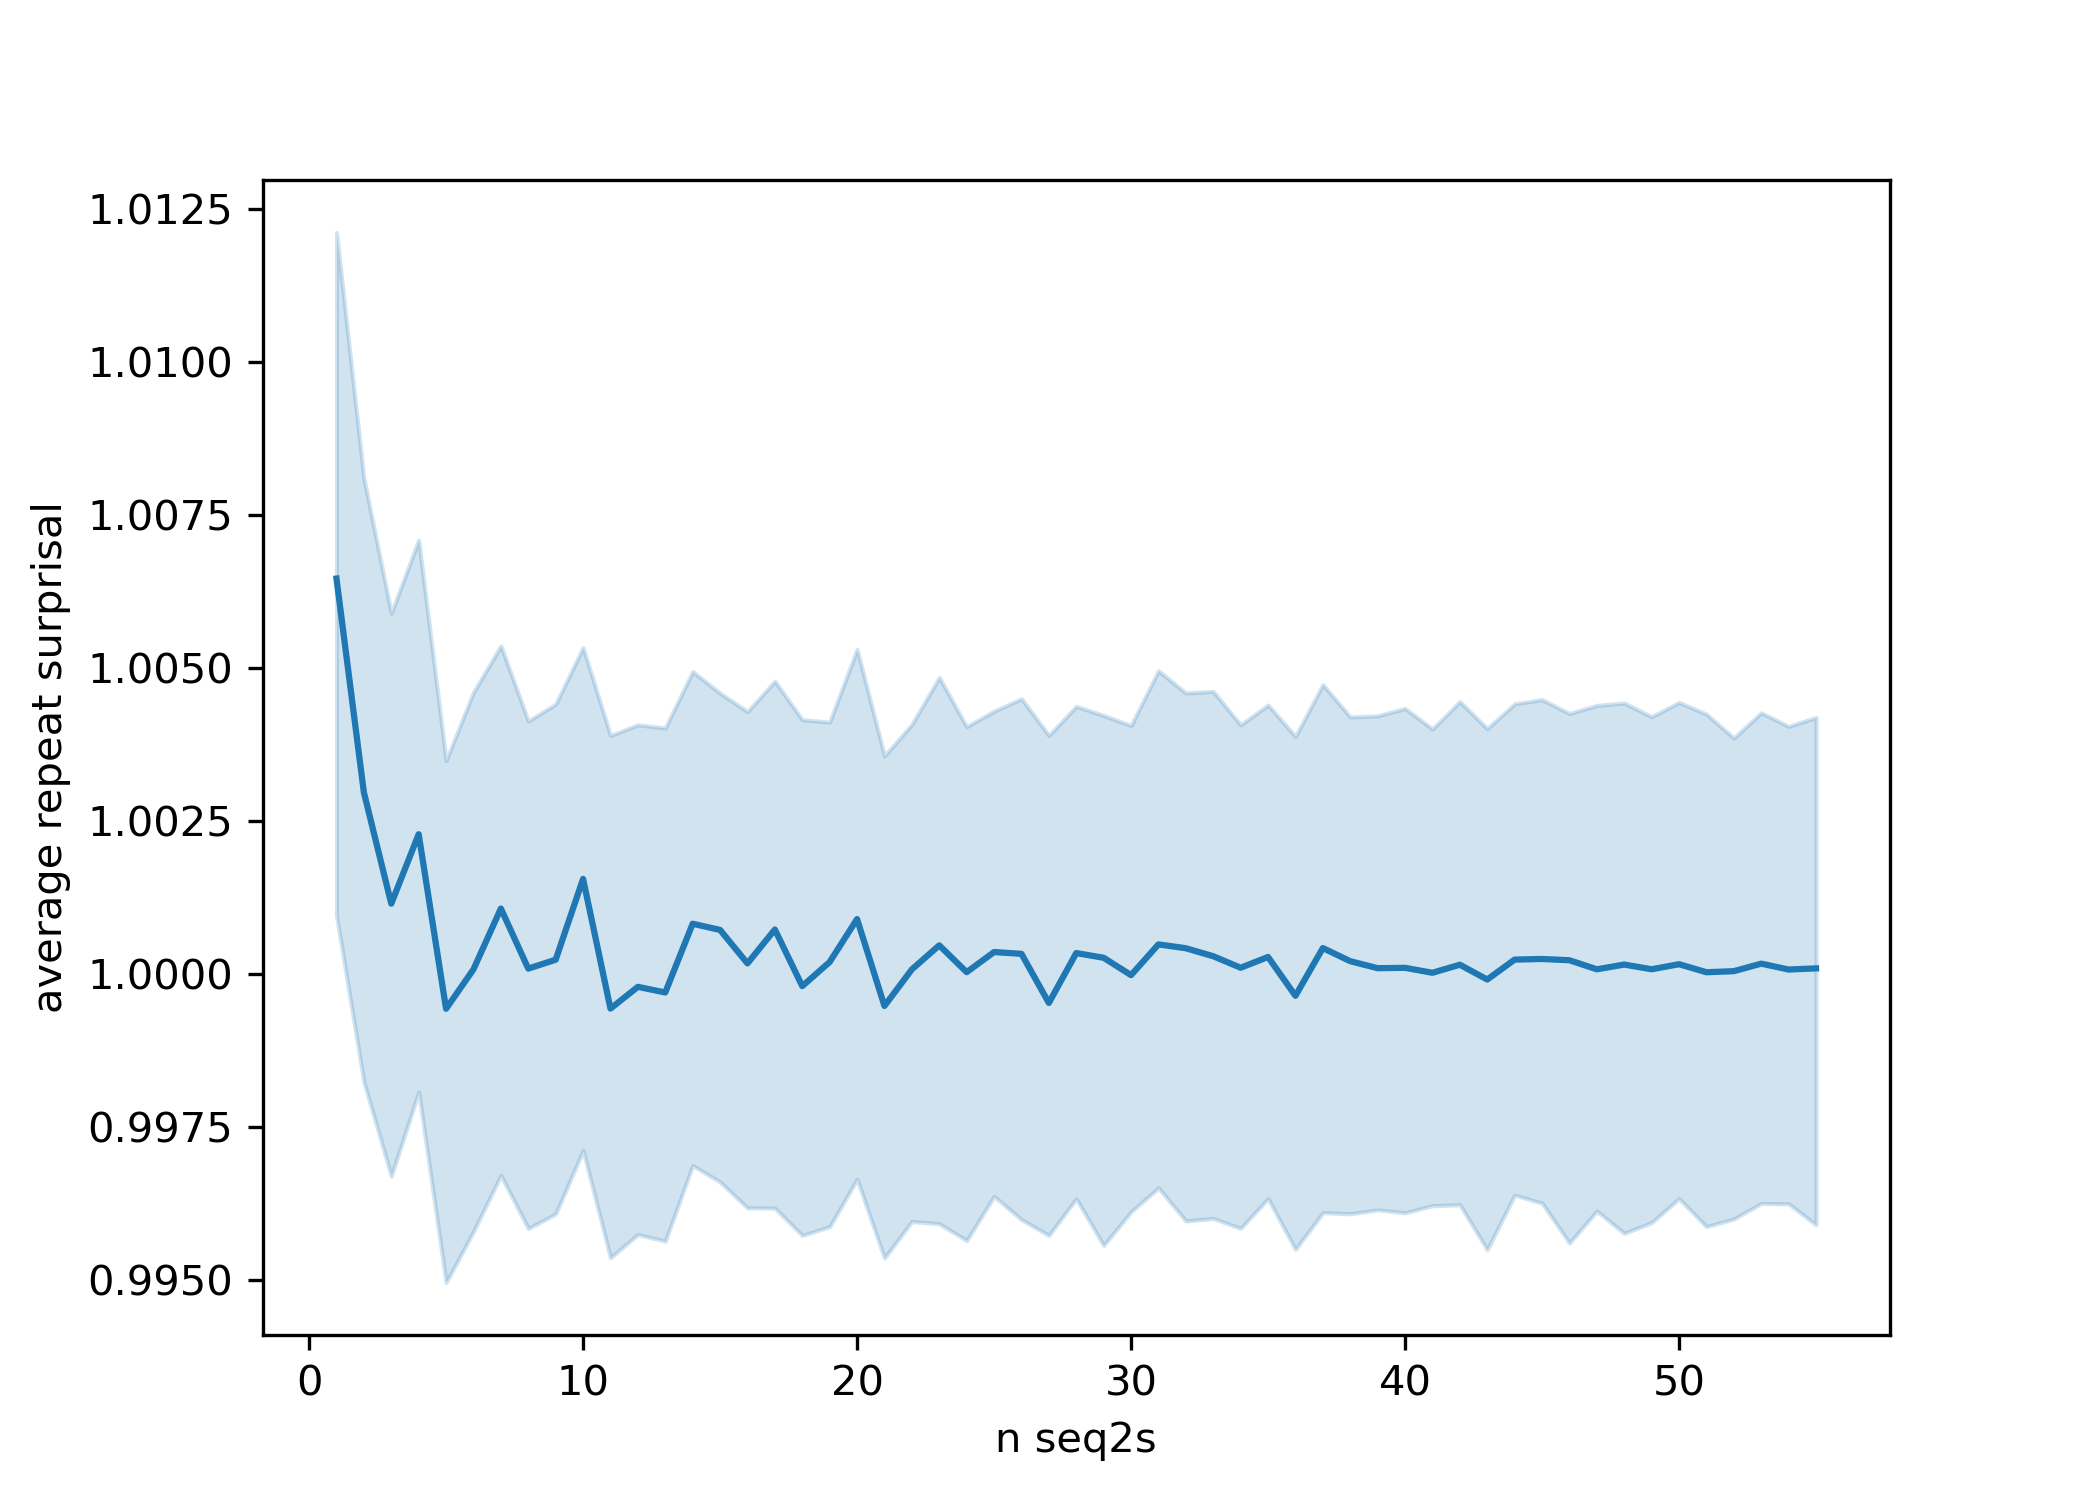
\includegraphics[width=.4\textwidth]{appendix/repeat_surprisal_nseq2_closeup.png}}
  \caption{Average surprisal of the median of control-sentences dependent on the amount of control-sentences used (a,b). Average repeat surprisal dependent on the amount of control-sequences used (c,d). Experiments were repeated 50 times.}
  \label{fig:rs_10_controls}
\end{figure}


\subsection{Sampling of Synonyms}\label{app:syn_sampling}

In order to create the SYN condition of \ref{exp:word_swap}, synonyms for the nouns verbs of our sentences are needed.

For sampling we created a synonym candidate list with help of \url{https://www.thesaurus.com/}, \parencite{miller_wordnet_1995} and \href{http://paraphrase.org}{PPDB} \parencite{pavlick_ppdb_2015} (accessed with code from \href{https://github.com/makcedward/nlpaug}{nlpaug}).
This synonym candidate list was proofread by at one (nonce-sentences) or two (wikitext sentences) native English speakers. The entire list of synonyms can be found \href{https://docs.google.com/spreadsheets/d/1H95LVB7VJXTtizHpGqHZp7Ky9NsPlMgj-W6yAFc6LOI/edit}{here}.

\begin{table} \centering
    \begin{threeparttable}
        \begin{tabular}{ p{0.39\linewidth} | c | c c c}
            \hline
            \thead{Sentence} & \thead{Target word} & \multicolumn{3}{c}{\thead{Synonyms}} \\
            \hline\hline
            the section on current routes adds nothing to the info . & section & part	& passage & paragraph \\
            \hline
            the section on current routes adds nothing to the info . & adds & appends	& supplements & \\
        \end{tabular}
        \caption{Example synonyms} \label{Tab:syn_sampling}
    \end{threeparttable}
\end{table}

We actively decided against generating these synonyms with LMs to avoid a circular argument:
In the hypothetical case in which synonyms are sampled with a LM we test our transformers on that LMs semantic knowledge of contextual synonyms, and not the human semantic knowledge of synonyms.
For instance, the generated synonyms may only are synonyms which are easily learned by LMs because of certain word distributions.
The tested transformers may as well easily pick up on these synonyms.
Subsequently, the tested transformers may have an easier time predicting these synonyms during our experiment, whilst there may exist another class of synonyms which does not show such a property.
We thus would arrive at the wrong conclusion.


\subsection{Word-swap Experiment detailed Setup}\label{app:word_swap_setup}

\begin{itemize}
    \item[RPT] All 60 sentences (sec. \ref{met:sentences_used}) are used to create 60 test sequences. For each test sequence, one sentence is used as encoding- and test-sentence (such that encoding- and test-sentence are the same).
    \item[SYN] For each of the 60 sentences synonyms were sampled for both the marked verb and noun. The 60 original sentences are used as encoding-sentence. They are paired with a test-sentence which is the same except for the word at the marked position: instead of the original word, a semantically fitting synonym is inserted.
    \item[ARB] As in SYN, the 60 original sentences are used as encoding-sentences. They are paired with a test-sentence in which the marked word is replaced with an arbitrary word within the same part-of-speech category as the original word. The arbitrary nouns and verbs sampled from a list of 200 verbs and 300 nouns respectively. These lists are taken from the nonce-dataset \cite{linzen_assessing_2016}. For each original sentence, $10$ verbs and $10$ nouns are sampled, for a total of $60 \dot 10$ measures.
\end{itemize}
In each condition 10 pairwise-different control-sentences are sampled from the then remaining original $59$ sentences to construct the control sequences.


\subsection{Repeat Experiment: Generalization across transformers}

\begin{figure}[H]
    \centering
    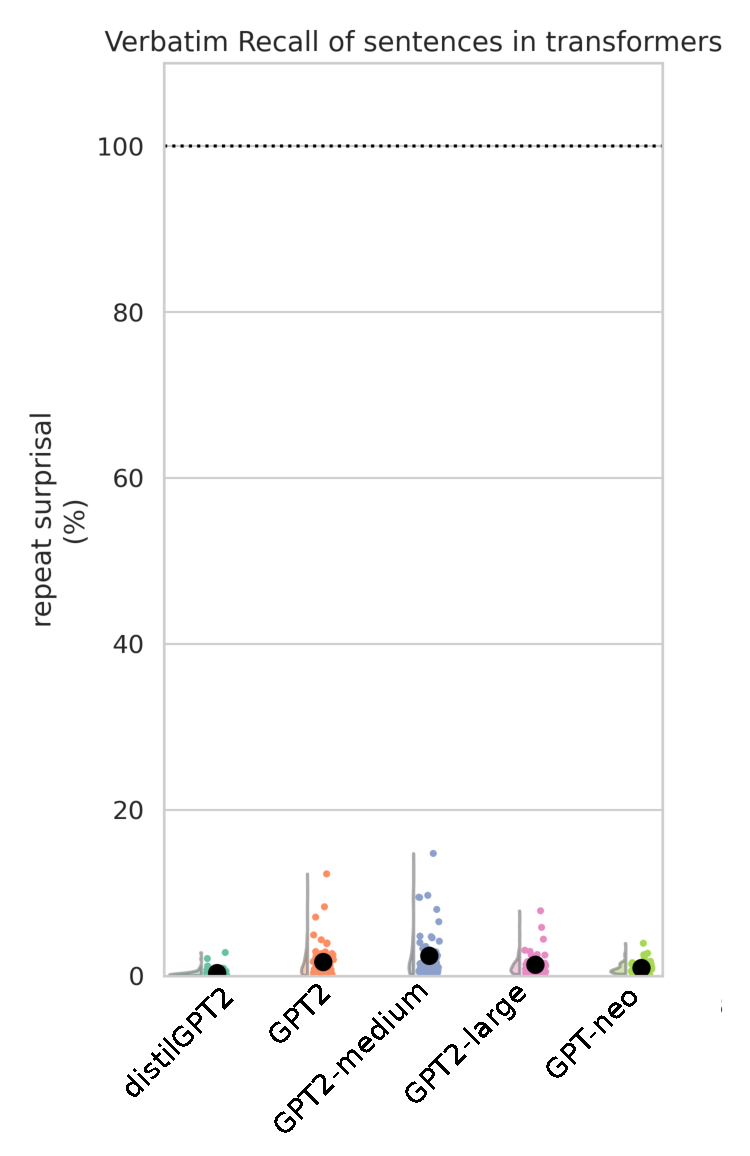
\includegraphics[width=0.5\textwidth]{experiments/repeat_surprisal_all.pdf}
    \caption{Repeat surprisal for different transformer models for verbatim repetition of sentences ($N = 60$). The Y axis shows the repeat surprisal as percentage. The ``raincloud plot'' \parencite{allen_raincloud_2019} shows the distribution of repeat surprisal as kernel density estimate (left). The points (right) are the actual repeat surprisal values for each measure. The black point (right) indicates the mean. Bootstrap $95\%$ confidence intervals are plotted around the mean, but are not visible due the consistency of the repeat surprisal in this experiment.}
    \label{fig:repeat_all}
\end{figure}


\subsection{Repeat Experiment: How M0, M1, M2 and M3 can account for results} \label{app:repeat_null_explanation}

\textbf{M0} fWM, together with the transformers ability to create syntactically coherent sentences suffice to explain the result: every word in the test-sentence is in prior context, and has its probability significantly increased by the M0 fWM. The model now selects the right words based on the syntactic plausibility at each position.
\textbf{M1} fWM heightens the probability of the continuation of the longest to current context matching sequence in the past context.
This results in an increase of probability for exactly the repeated word.
\textbf{M2} fWM operates as M1 fWM, additionally increasing probabilities of words within the same POS-category as the continued word.
Since probabilities for the continued word itself are still increased, the low repeat surprisal is conceivable.
\textbf{M3} fWM works analogous to M2 fWM just increasing probabilities for synonyms of the continued word instead of within-POS-category words.


\subsection{Word-swap experiment: Generalization across transformers}

\begin{figure}[H]
    \centering
    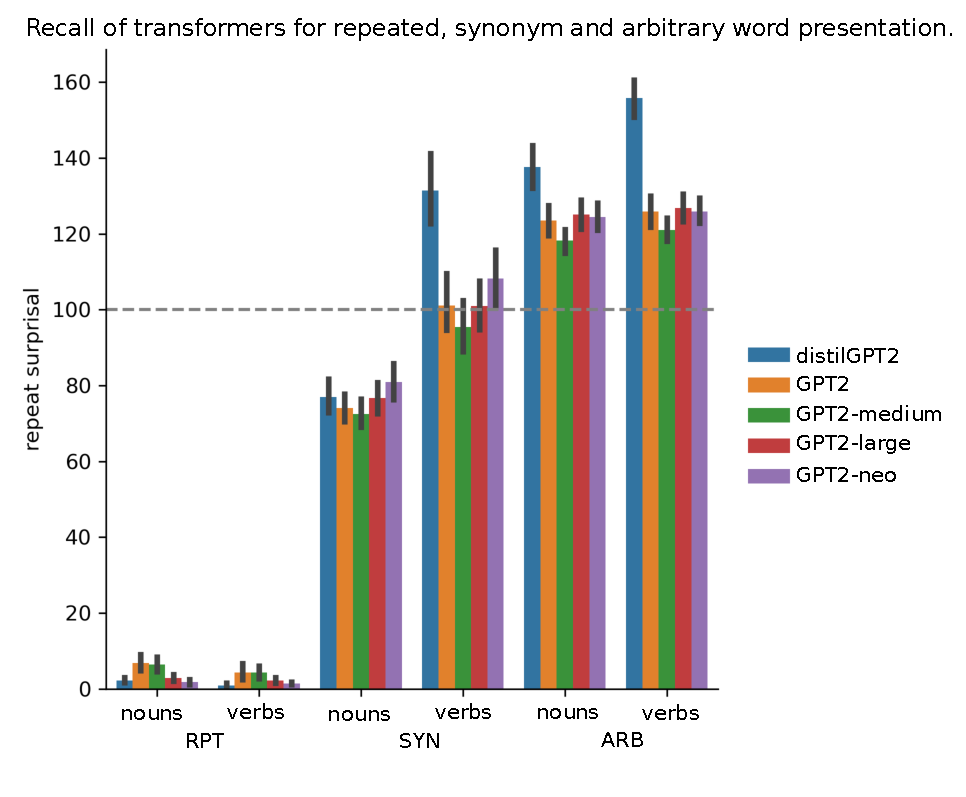
\includegraphics[width=\textwidth]{experiments/word_swap_all.pdf}
    \caption{Bar plot of repeat surprisal for the RPT, SYN and ARB conditions in the word swap experiment across transformers. The bars indicates the mean, the whiskers denote the $95\%$ confidence interval. In most conditions the transformers perform very similar to each other.}
    \label{fig:word_swap_all}
\end{figure}
